\subsection{V1}
The video is recorded at 29 fps. For simplicity only detections of the right side of the traffic are
taken into account in this video. In this experiments frames 36-79 of video V1 are shown, as it includes some curios situations.
\subsection{V1 -- GM-PHD with constant detection probability}
The measurements for GM-PHD filter with constant detection probability are obtained by the YOLO object detection
model. The parameters' values are displayed in Table \ref{tab:E1-V1-S0}.
\begin{table}[!h]
    \centering
    \begin{tabular}{|c|c|c|c|c|c|}
        \hline
        $P_{D}$ & $P$ & $\sigma_{\upsilon}$ & $\sigma_{\epsilon}$ & $T_p$ & $T_{YOLO}$ \\ \noalign{\hrule height 1.5pt}
        0.9 & $diag(600,600,600,600)$ & 0.1 & 150 & 0.1 & 0.3\\
        \hline
    \end{tabular}
    \caption{The parameter settings for experiment E1-V1 with constant detection probability.}
    \label{tab:E1-V1-S0}
\end{table}

Figure \ref{fig:E1-V1-S0} shows some highlights of the GM-PHD filter with the constant detection probability.
\begin{itemize}
    \item \textbf{\ref{fig:E1-V1-S0:01}:} This is the starting frame, where four cars were previously detected, thus they became our observed targets. In the distance we see that one more car was detected by YOLO, but it did not cross any spawning point, so it does not count into observed targets.
    \item \textbf{\ref{fig:E1-V1-S0:02}:} Another car is approaching to the scene and should be initialized soon. The YOLO model is not able to always detect all desired objects, as it happened here with the left distanced car. As the detection probality is 0.9, this target did not survive the pruning step and is lost now.
    \item \textbf{\ref{fig:E1-V1-S0:03}:} The previously lost car is detected again, but does not belong to the set of observed targets furthermore.
    \item \textbf{\ref{fig:E1-V1-S0:04}:} The new car crossed the spawning point, but the YOLO model was not able to detect this kind of car for many frames in a row, thus this car is not tracked at all.
    \item \textbf{\ref{fig:E1-V1-S0:05}:} Two cars on the right were not detected again. But this time onw of the targets was able to survive, so we continue to track at least one of the cars.
    \item \textbf{\ref{fig:E1-V1-S0:06}:} The previously undetected cars are detected again and both cars are tracked again.
    \item \textbf{\ref{fig:E1-V1-S0:07}:} Another car arrives to the scene and this time it is successfully detected and initialized.
    \item \textbf{\ref{fig:E1-V1-S0:08}:} Even though all six cars are detected by YOLO, only three targets appear in the scene. One of the targets covers two cars at once so we can guess that four out of six targets are covered by the GM-PHD filter.
\end{itemize}

In Graph \ref{gr:E1-V1-S0} it is clearly seen that even though the number of targets is increasing, the misdetection of the YOLO model causes the targets loss. The "All targets in set" line is fully covered by the blue line, thus the targets are absolutely lost, thus they can not be reborn by a measurement.

This experiment shows us that the GM-PHD filter is able to accurately track the position of objects. With detection probablity $p_D = 0.9$ and without modified pruning technique, the filter is very sensitive to the output of object detector and if YOLO is not able to detect all desired objects, targets could be easily lost.

\begin{figure}[H]
    \centering
    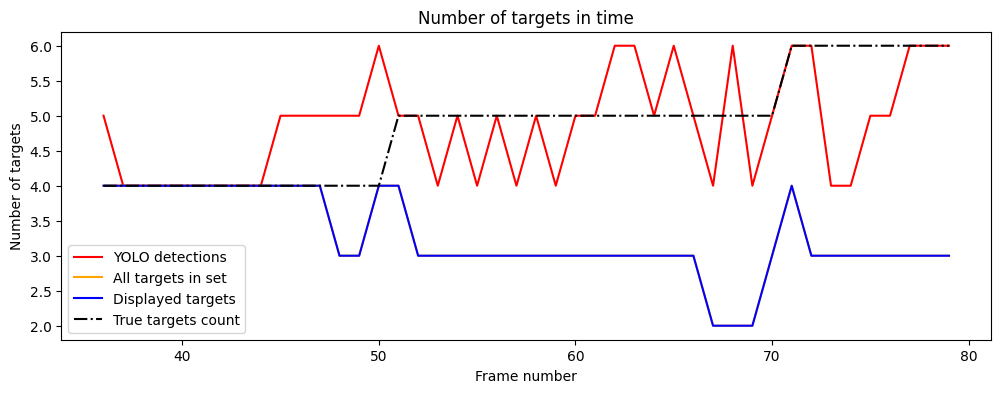
\includegraphics[width=\linewidth]{../../../experiments/E1/V1/noPd/staticPd_det}
    \caption{Development chart of number of detected targets, targets in filter's queue, displayed targets and true targets' count.}
    \label{gr:E1-V1-S0}
\end{figure}

\begin{figure}[H]
    \centering
    \begin{subfigure}{0.48\textwidth}
        \centering
        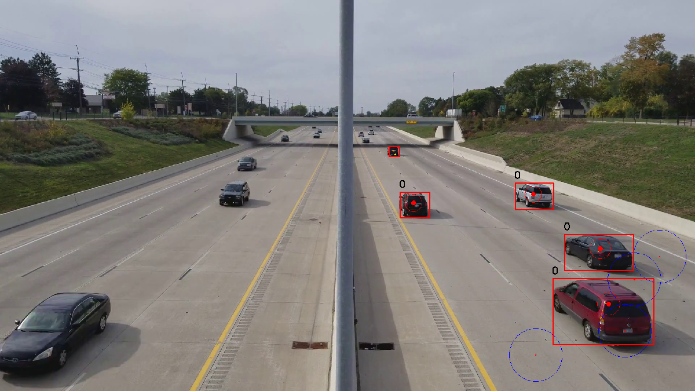
\includegraphics[width=\linewidth]{../../../experiments/E1/V1/noPd/36}
        \caption{Frame number: 36.}
        \label{fig:E1-V1-S0:01}
    \end{subfigure}
    \begin{subfigure}{0.48\textwidth}
        \centering
        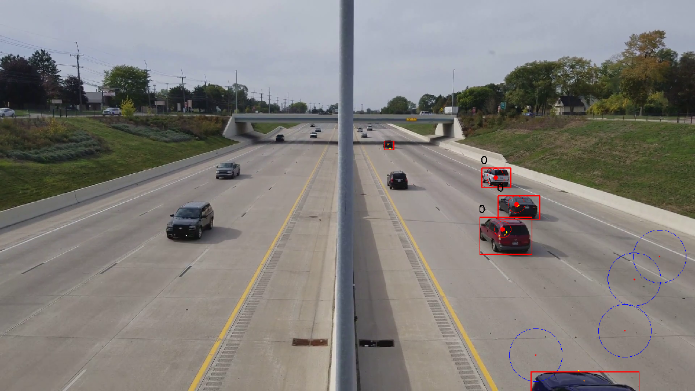
\includegraphics[width=\linewidth]{../../../experiments/E1/V1/noPd/48}
        \caption{Frame number: 48.}
        \label{fig:E1-V1-S0:02}
    \end{subfigure}
    \\
    \begin{subfigure}{0.48\textwidth}
        \centering
        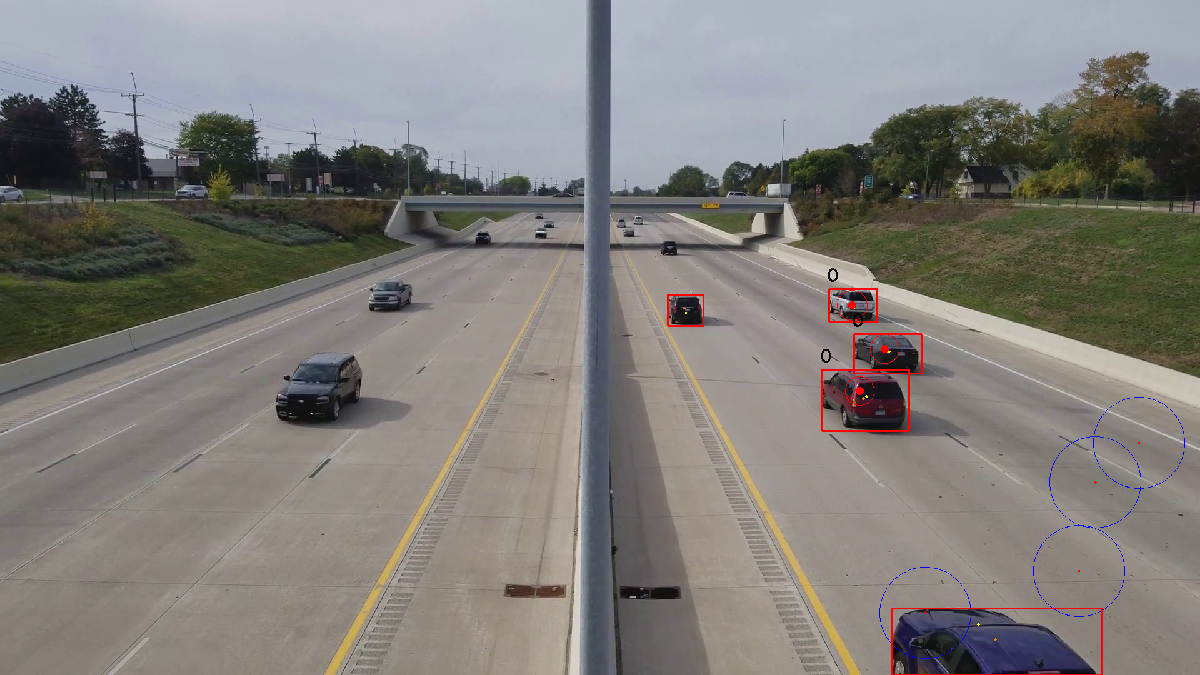
\includegraphics[width=\linewidth]{../../../experiments/E1/V1/noPd/49}
        \caption{Frame number: 49.}
        \label{fig:E1-V1-S0:03}
    \end{subfigure}
    \begin{subfigure}{0.48\textwidth}
        \centering
        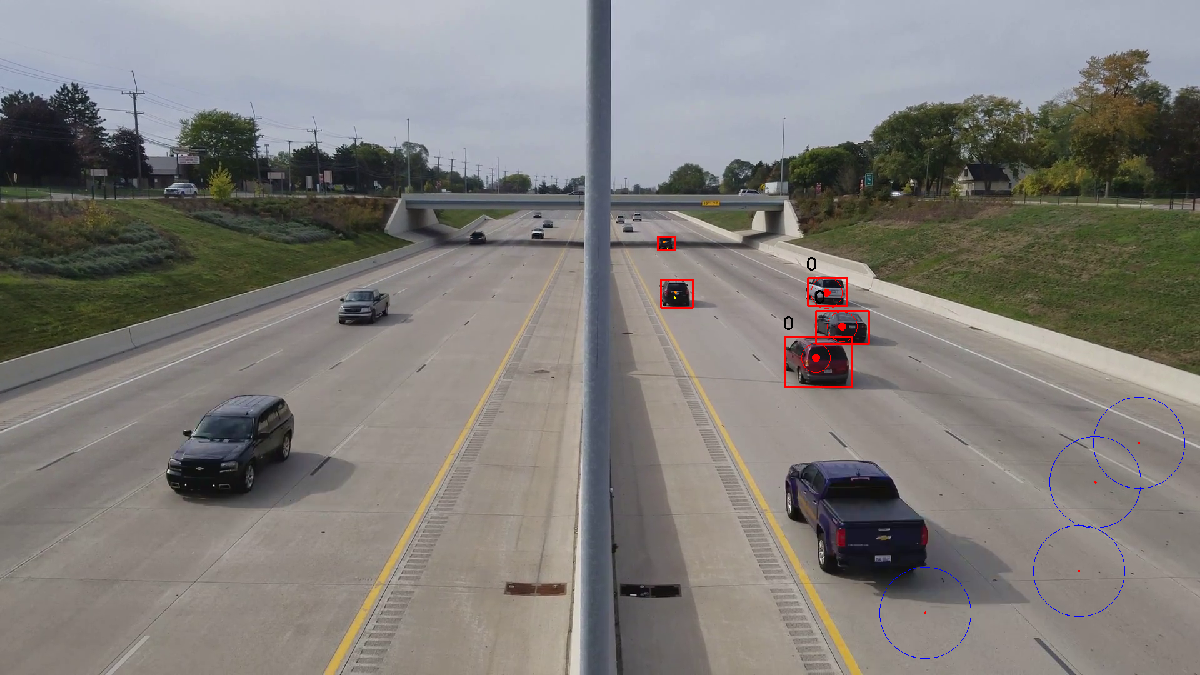
\includegraphics[width=\linewidth]{../../../experiments/E1/V1/noPd/56}
        \caption{Frame number: 56.}
        \label{fig:E1-V1-S0:04}
    \end{subfigure}
    \\
    \begin{subfigure}{0.48\textwidth}
        \centering
        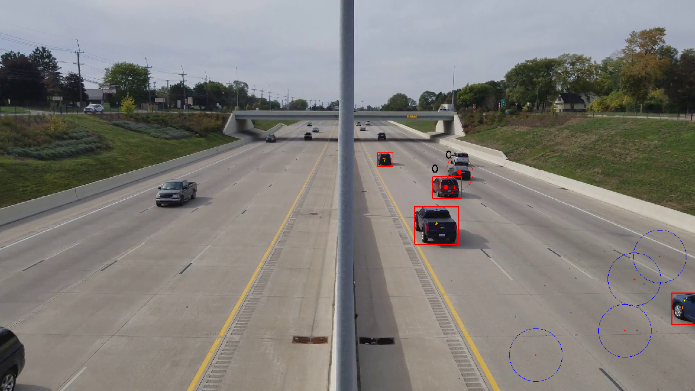
\includegraphics[width=\linewidth]{../../../experiments/E1/V1/noPd/67}
        \caption{Frame number: 67.}
        \label{fig:E1-V1-S0:05}
    \end{subfigure}
    \begin{subfigure}{0.48\textwidth}
        \centering
        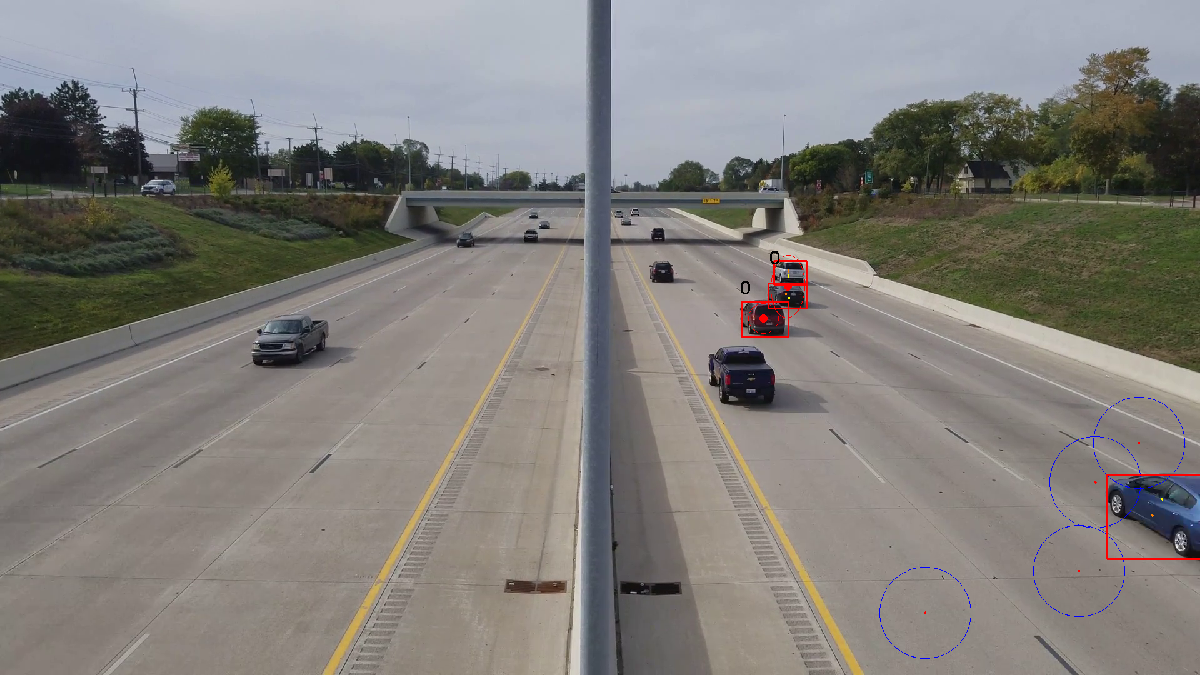
\includegraphics[width=\linewidth]{../../../experiments/E1/V1/noPd/69}
        \caption{Frame number: 69.}
        \label{fig:E1-V1-S0:06}
    \end{subfigure}
    \\
    \begin{subfigure}{0.48\textwidth}
        \centering
        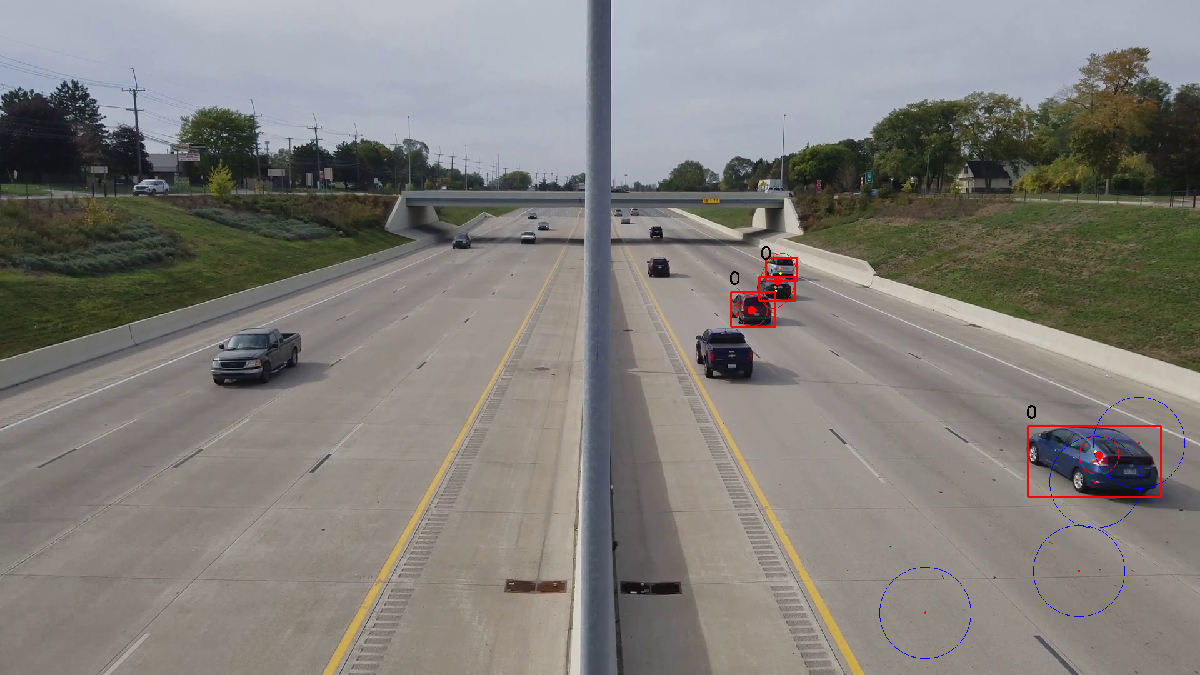
\includegraphics[width=\linewidth]{../../../experiments/E1/V1/noPd/73}
        \caption{Frame number: 73.}
        \label{fig:E1-V1-S0:07}
    \end{subfigure}
    \begin{subfigure}{0.48\textwidth}
        \centering
        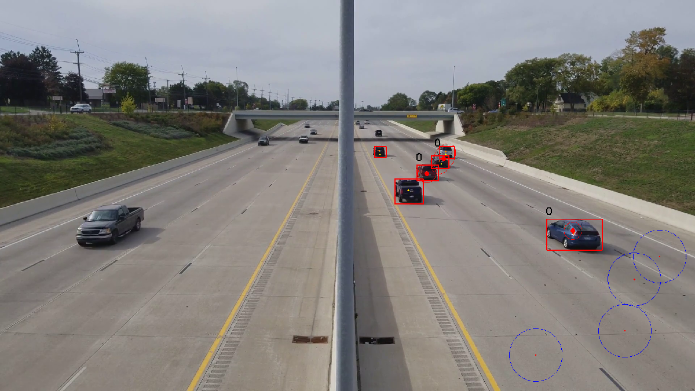
\includegraphics[width=\linewidth]{../../../experiments/E1/V1/noPd/79}
        \caption{Frame number: 79.}
        \label{fig:E1-V1-S0:08}
    \end{subfigure}
    \caption{Image sequence of tracked objects using GM-PHD filter with constant detection probability.}
    \label{fig:E1-V1-S0}
\end{figure}

\subsection{V1 -- GM-PHD with dynamic detection probability}
Following experiments test GM-PHD filter with the dynamic detection probability and the modified pruning on the video \textit{V1}.
\subsubsection{S1 -- YOLO + YOLO}
This experiment uses settings \textit{S1}, i.e, the YOLO model provides with both object detection bboxes and segmentation masks.
The parameter settings are shown in Table \ref{tab:E1-V1-S1}.
\begin{table}[H]
    \centering
    \begin{tabular}{|c|c|c|c|c|c|c|c|c|}
        \hline
        $P_{D,k}(x)$ & $P$ & $\sigma_{\upsilon}$ & $\sigma_{\epsilon}$ & $T_H$ & $T_d$ & $T_p$ & $T_l$ & $T_{YOLO}$ \\ \noalign{\hrule
        height 1.5pt}
        0.3 & $diag(600,600,600,600)$ & 0.1 & 150 & 1 & 3 & 0.1 & 0.01 & 0.3\\
        \hline
    \end{tabular}
    \caption{The parameter settings for experiment E1-V1-S1 with dynamic detection probability.}
    \label{tab:E1-V1-S1}
\end{table}

Figure \ref{fig:E1-V1-S1} shows the performance of the GM-PHD filter with the dynamic detection probability with settings \textit{S1}.
\begin{itemize}
    \item \textbf{\ref{fig:E1-V1-S1:01}:} As in previous experiment the first frame starts with four cars that were previously detected. The car that is far away is detected, but not initialized, as it have not crossed any spawning point.
    \item \textbf{\ref{fig:E1-V1-S1:02}:} In the frame 48, the left distanced car was not detected as in previous experiment. But due to the high detection probability and modified pruning, the target is able to survive.
    \item \textbf{\ref{fig:E1-V1-S1:03}:} The previously undetected car is detected again and the target survives even with misdetection in previous frames.
    \item \textbf{\ref{fig:E1-V1-S1:04}:} The new car crossed the spawning point, but the YOLO model is not able to detect this vehicle for many consecutive frames, thus this car is not initialized.
    \item \textbf{\ref{fig:E1-V1-S1:05}:} Two cars on the right are not detected again but targets survive.
    \item \textbf{\ref{fig:E1-V1-S1:06}:} The previously undetected cars are detected again and both targets get their measurements increasing their weight.
    \item \textbf{\ref{fig:E1-V1-S1:07}:} Another car arrives to the scene, and it is successfully initialized.
    \item \textbf{\ref{fig:E1-V1-S1:08}:} The undetected car on the left caught up other targets. As a result of this is initializing this target, even though it is misdetected most of the time. And so we have six true targets and also six tracked targets.
\end{itemize}

The graph \ref{gr:E1-V1-S1} presents better performance of the GM-PHD filter. Even though not all the targets are displayed when they should, most of the time, there are more targets is a queue that do not have weight high enough to be displayed. As soon as these targets get their measurements, their weight increases and are back on the scene.

Not only the number of displayed targets is closer to the true targets count, but also targets waiting in the queue exceeds the true count, so we are aware of the potential targets, that can appear in the scene.

\begin{figure}[H]
    \centering
    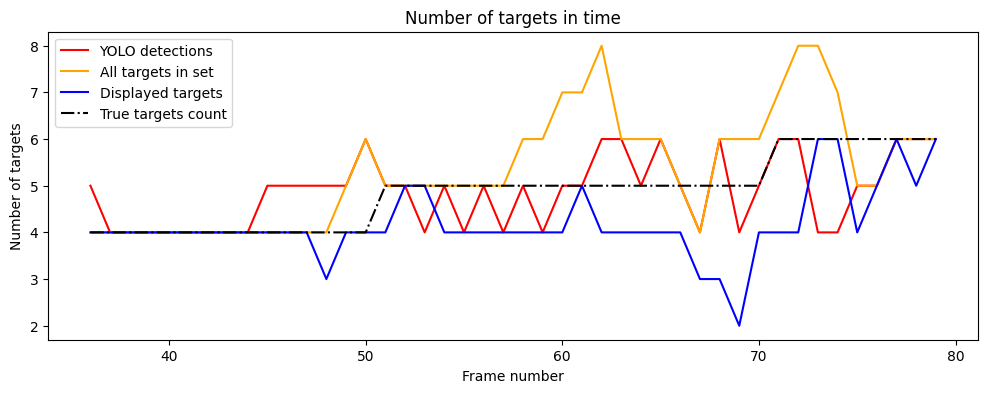
\includegraphics[width=\linewidth]{../../../experiments/E1/V1/YOLO/yolo_det}
    \caption{Development chart of number of detected targets, targets in filter's queue, displayed targets and true targets' count.}
    \label{gr:E1-V1-S1}
\end{figure}

\begin{figure}[H]
    \centering
    \begin{subfigure}{0.48\textwidth}
        \centering
        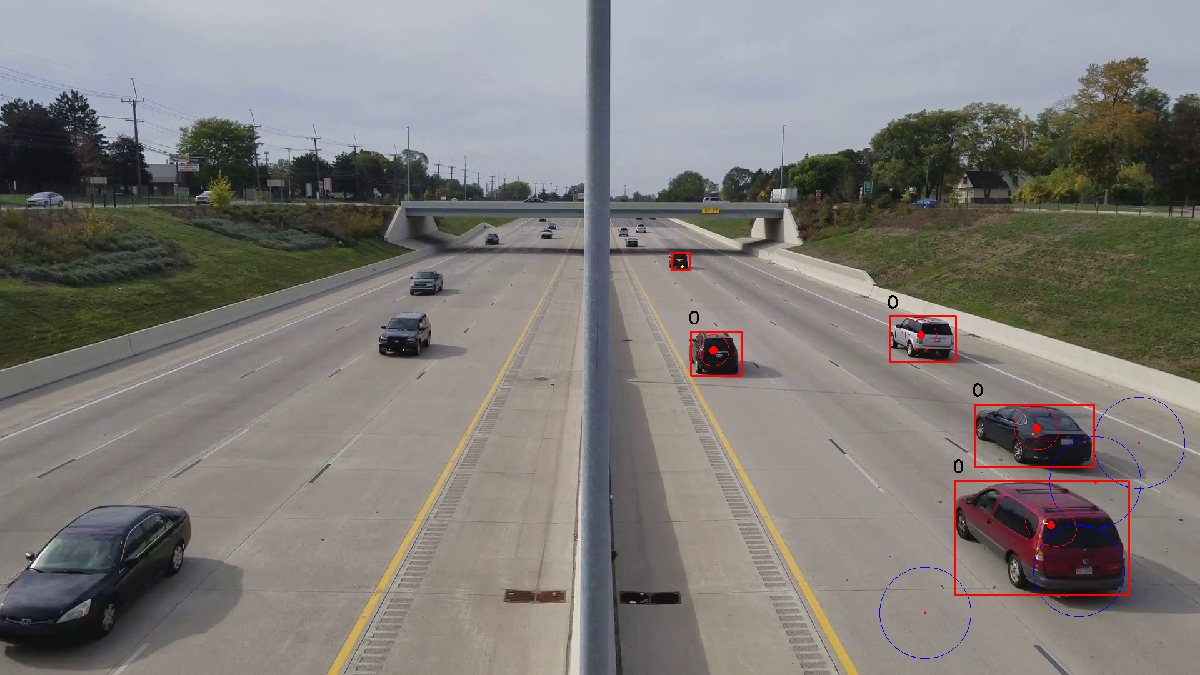
\includegraphics[width=\linewidth]{../../../experiments/E1/V1/YOLO/36}
        \caption{Frame number: 36.}
        \label{fig:E1-V1-S1:01}
    \end{subfigure}
    \begin{subfigure}{0.48\textwidth}
        \centering
        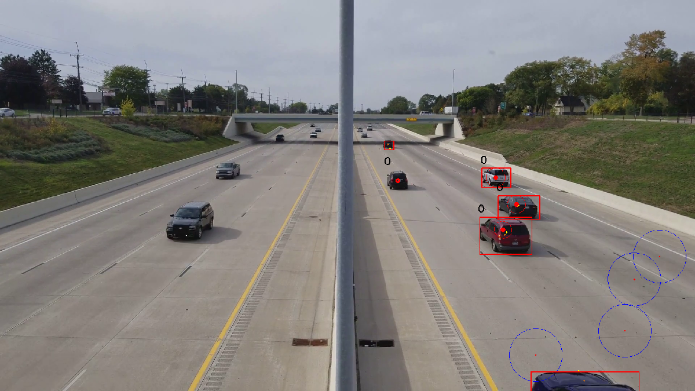
\includegraphics[width=\linewidth]{../../../experiments/E1/V1/YOLO/48}
        \caption{Frame number: 48.}
        \label{fig:E1-V1-S1:02}
    \end{subfigure}
    \\
    \begin{subfigure}{0.48\textwidth}
        \centering
        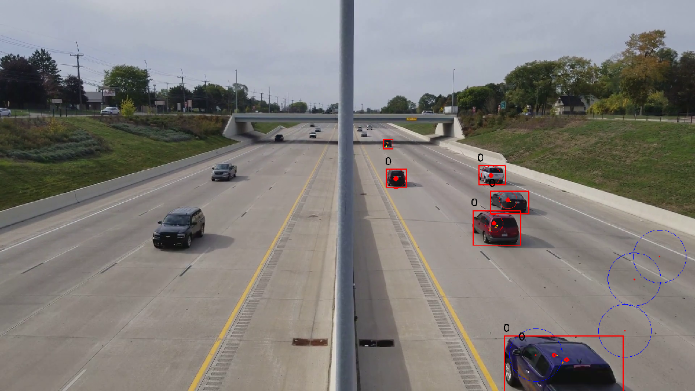
\includegraphics[width=\linewidth]{../../../experiments/E1/V1/YOLO/50}
        \caption{Frame number: 50.}
        \label{fig:E1-V1-S1:03}
    \end{subfigure}
    \begin{subfigure}{0.48\textwidth}
        \centering
        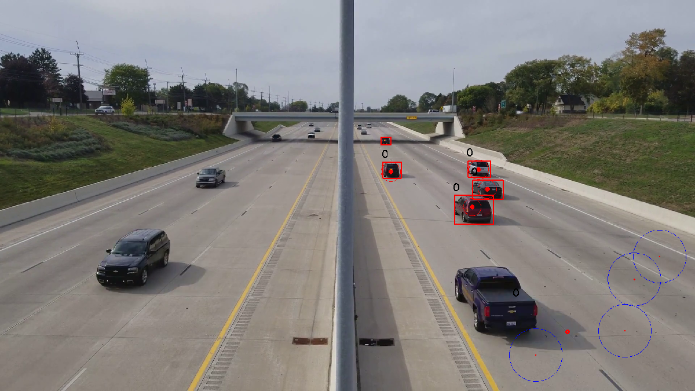
\includegraphics[width=\linewidth]{../../../experiments/E1/V1/YOLO/56}
        \caption{Frame number: 56.}
        \label{fig:E1-V1-S1:04}
    \end{subfigure}
    \\
    \begin{subfigure}{0.48\textwidth}
        \centering
        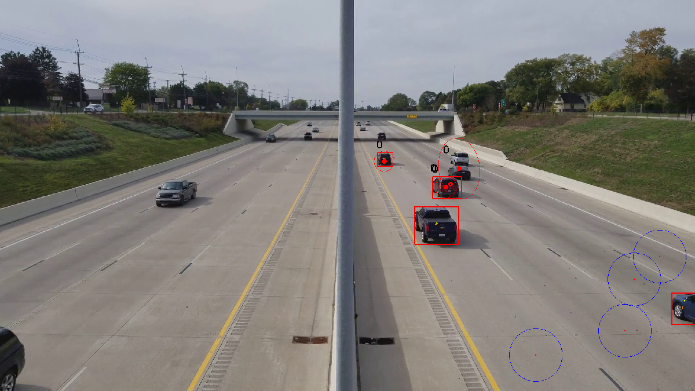
\includegraphics[width=\linewidth]{../../../experiments/E1/V1/YOLO/67}
        \caption{Frame number: 67.}
        \label{fig:E1-V1-S1:05}
    \end{subfigure}
    \begin{subfigure}{0.48\textwidth}
        \centering
        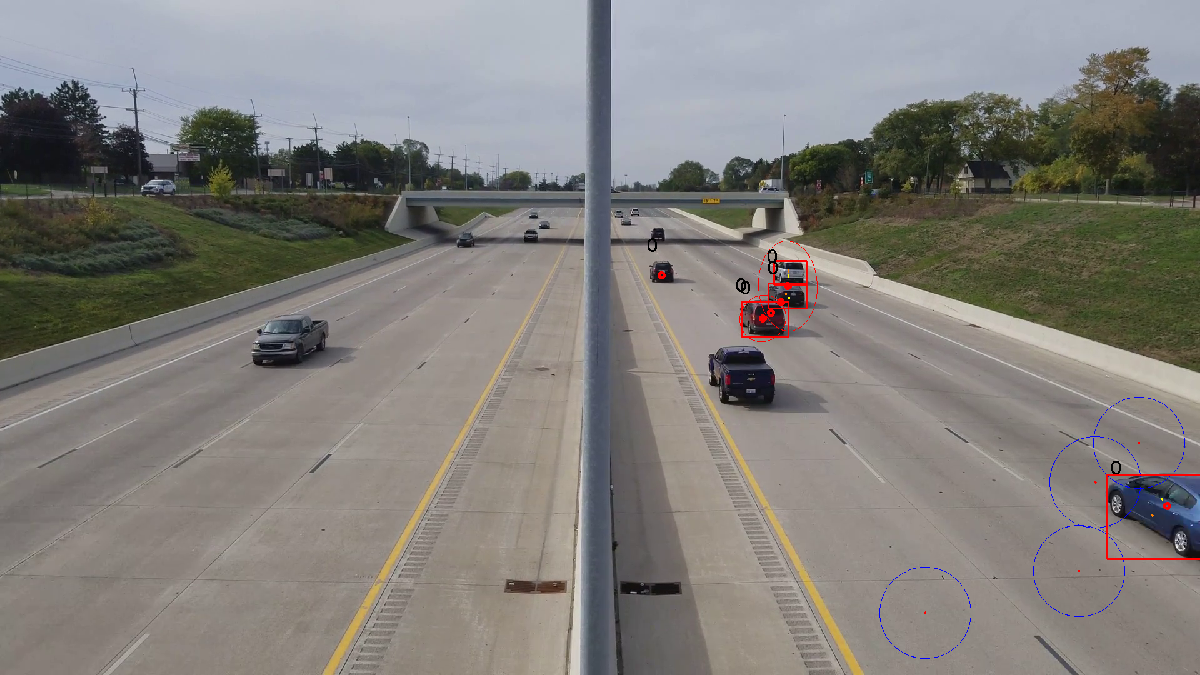
\includegraphics[width=\linewidth]{../../../experiments/E1/V1/YOLO/69}
        \caption{Frame number: 69.}
        \label{fig:E1-V1-S1:06}
    \end{subfigure}
    \\
    \begin{subfigure}{0.48\textwidth}
        \centering
        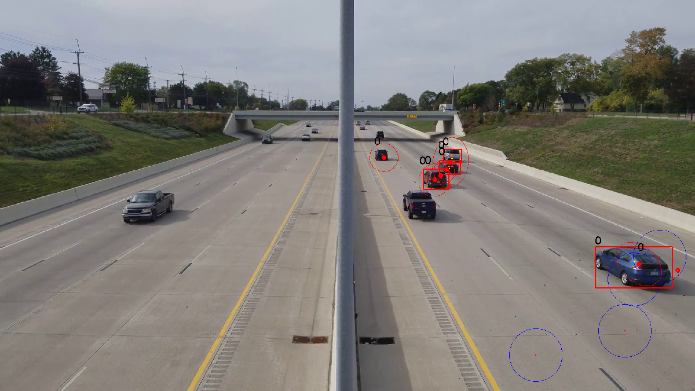
\includegraphics[width=\linewidth]{../../../experiments/E1/V1/YOLO/73}
        \caption{Frame number: 73.}
        \label{fig:E1-V1-S1:07}
    \end{subfigure}
    \begin{subfigure}{0.48\textwidth}
        \centering
        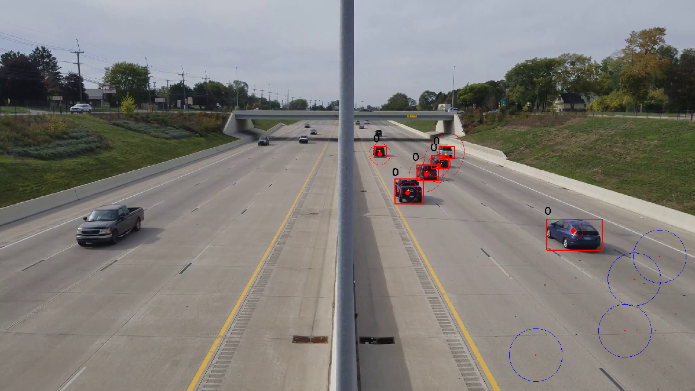
\includegraphics[width=\linewidth]{../../../experiments/E1/V1/YOLO/79}
        \caption{Frame number: 79.}
        \label{fig:E1-V1-S1:08}
    \end{subfigure}
    \caption{Image sequence of tracked objects using GM-PHD filter with dynamic detection probability and YOLO only.}
    \label{fig:E1-V1-S1}
\end{figure}







\subsubsection{S2 -- YOLO + SAM}
This experiment employs configuration \textit{S2}, wherein the YOLO model furnishes objects' bounding boxes and the SAM model furnishes segmentation masks.
The parameter configurations can be found in Table \ref{tab:E1-V1-S2}.
\begin{table}[H]
    \centering
    \begin{tabular}{|c|c|c|c|c|c|c|c|c|}
        \hline
        $P_{D,k}(x)$ & $P$ & $\sigma_{\upsilon}$ & $\sigma_{\epsilon}$ & $T_H$ & $T_d$ & $T_p$ & $T_l$ & $T_{YOLO}$ \\ \noalign{\hrule
        height 1.5pt}
        0.3 & $diag(600,600,600,600)$ & 0.1 & 150 & 1 & 3 & 0.1 & 0.01 & 0.3\\
        \hline
    \end{tabular}
    \caption{The parameter settings for experiment E1-V1-S2 with dynamic detection probability.}
    \label{tab:E1-V1-S2}
\end{table}

Figure \ref{fig:E1-V1-S2} illustrates the GM-PHD filter's performance with dynamic detection probability, employing settings \textit{S2}.
This sequence is very similar to the previous experiment. There are four targets at the beginning and they are tracked successfully the whole time. At frame \ref{fig:E1-V1-S2:06} two of the targets were not detected, but both survived. The YOLO model is not able to detect the fifth car, but it is initialized lated due to the other target.

The graph \ref{gr:E1-V1-S2} shows a better stability of number of tracked targets. This might be cased by the fact, that object detection YOLO model gives slightly different results than the object detection YOLO model with segmentation. The "All targets in set" orange line representing the number of targets in filter's queue is also more accurate to the true count, deflecting only be one target at maximum.

Settings \textit{S2} perform a little better than settings \textit{S1}. The number of tracked objects is closer to the true value.

\begin{figure}[H]
    \centering
    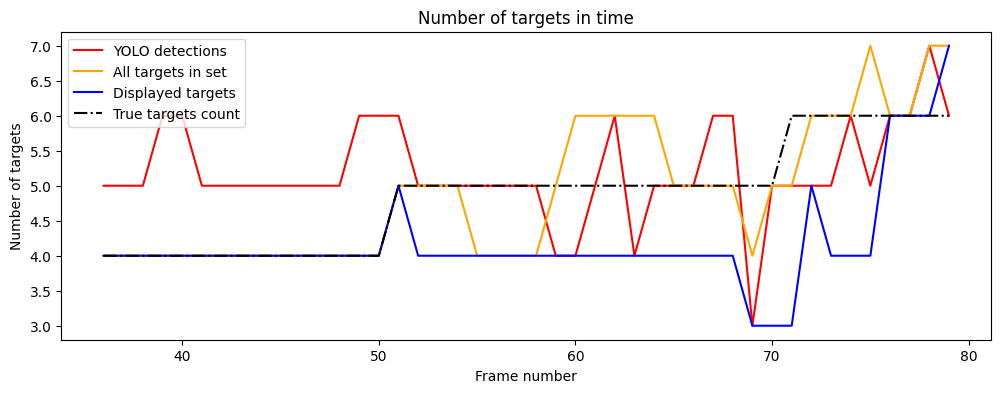
\includegraphics[width=\linewidth]{../../../experiments/E1/V1/SAM/sam_det}
    \caption{Development chart of number of detected targets, targets in filter's queue, displayed targets and true targets' count.}
    \label{gr:E1-V1-S2}
\end{figure}

\begin{figure}[H]
    \centering
    \begin{subfigure}{0.48\textwidth}
        \centering
        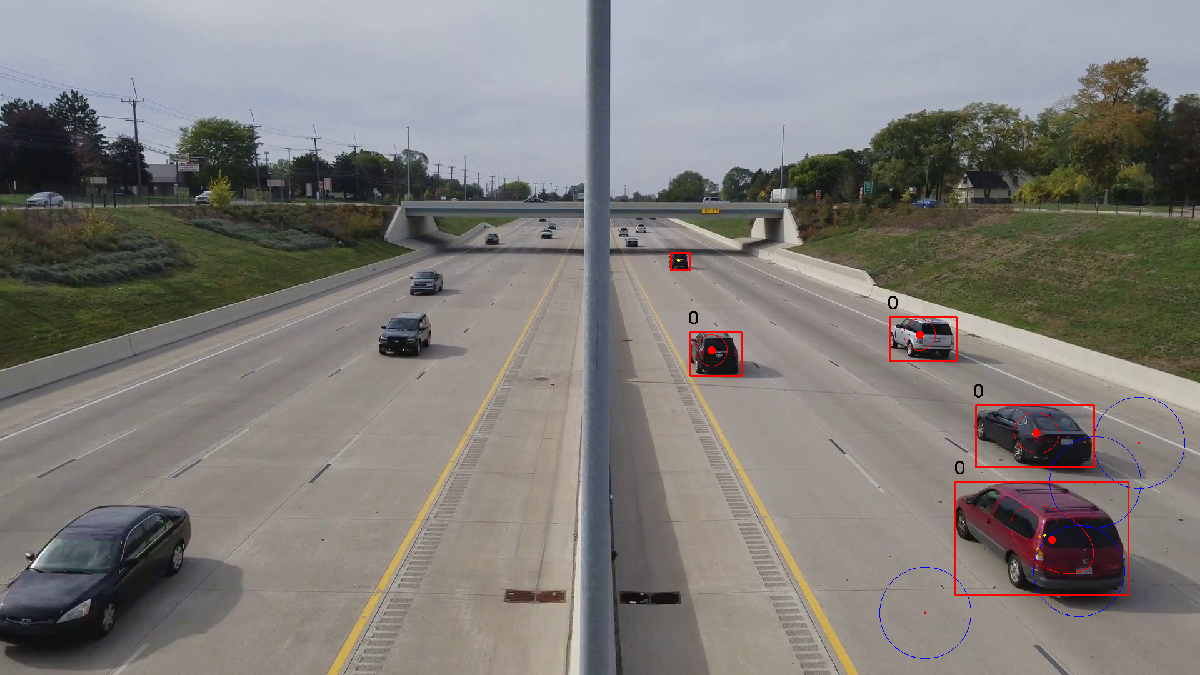
\includegraphics[width=\linewidth]{../../../experiments/E1/V1/SAM/36}
        \caption{Frame number: 36.}
        \label{fig:E1-V1-S2:01}
    \end{subfigure}
    \begin{subfigure}{0.48\textwidth}
        \centering
        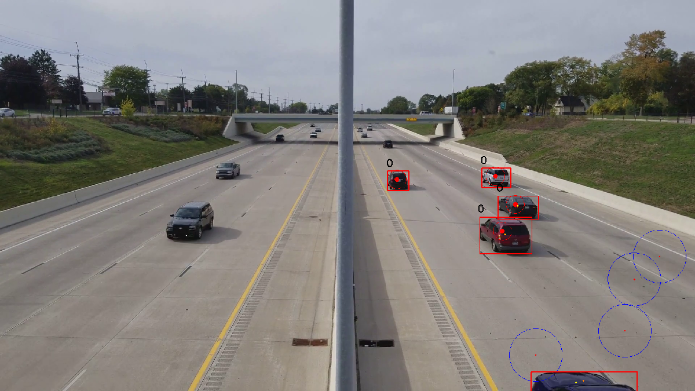
\includegraphics[width=\linewidth]{../../../experiments/E1/V1/SAM/48}
        \caption{Frame number: 48.}
        \label{fig:E1-V1-S2:02}
    \end{subfigure}
    \\
    \begin{subfigure}{0.48\textwidth}
        \centering
        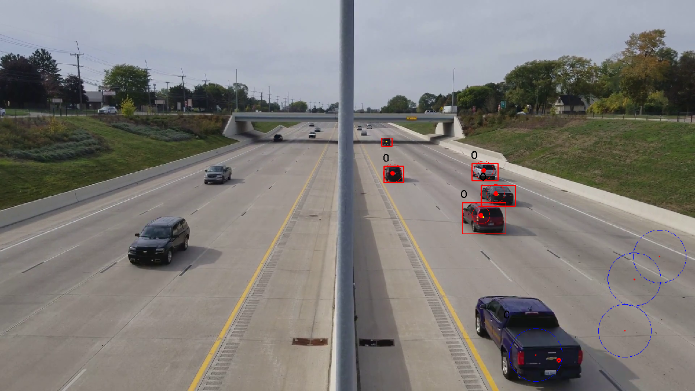
\includegraphics[width=\linewidth]{../../../experiments/E1/V1/SAM/53}
        \caption{Frame number: 53.}
        \label{fig:E1-V1-S2:03}
    \end{subfigure}
    \begin{subfigure}{0.48\textwidth}
        \centering
        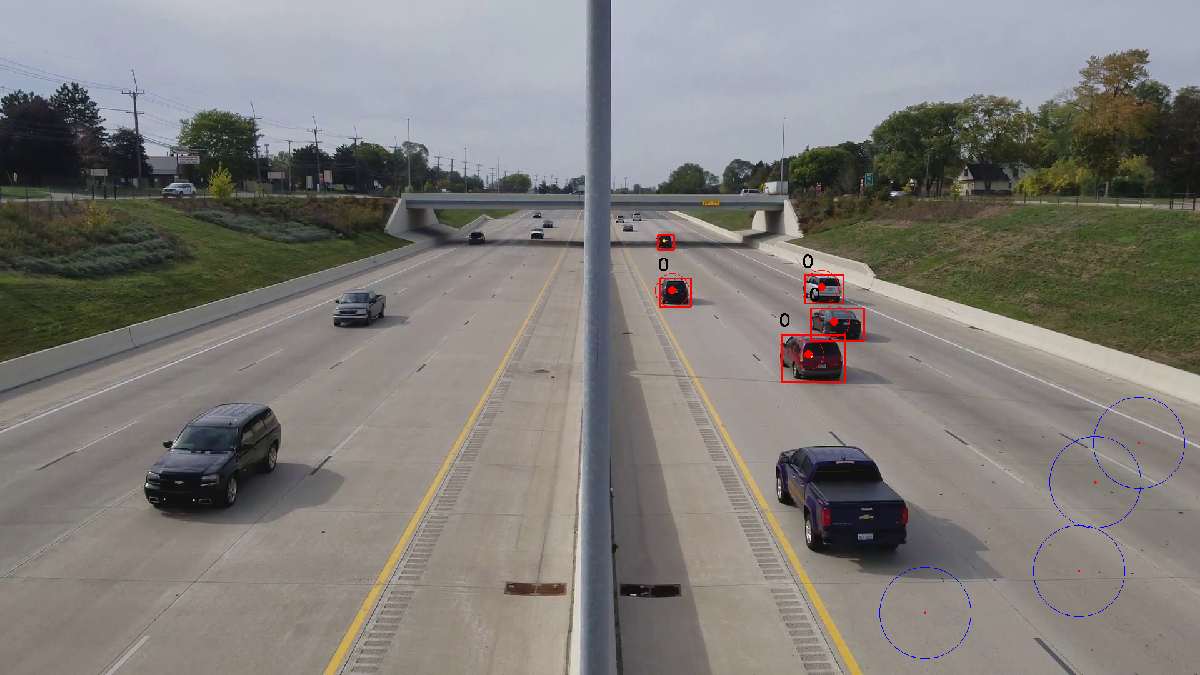
\includegraphics[width=\linewidth]{../../../experiments/E1/V1/SAM/57}
        \caption{Frame number: 57.}
        \label{fig:E1-V1-S2:04}
    \end{subfigure}
    \\
    \begin{subfigure}{0.48\textwidth}
        \centering
        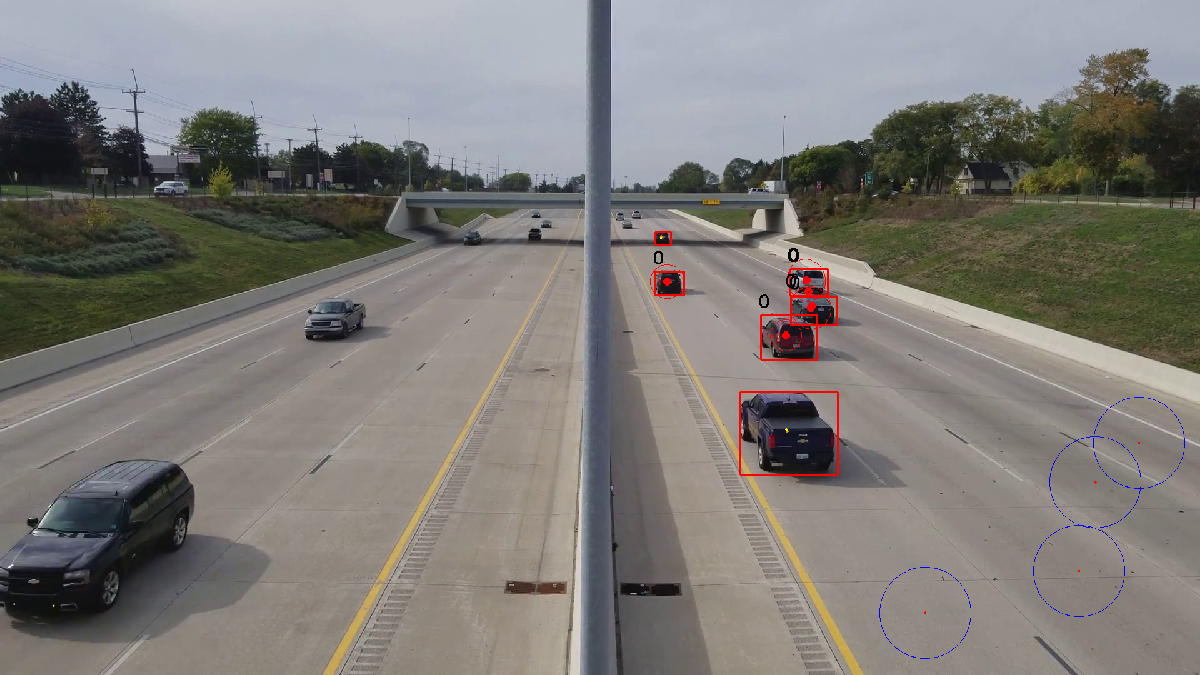
\includegraphics[width=\linewidth]{../../../experiments/E1/V1/SAM/62}
        \caption{Frame number: 62.}
        \label{fig:E1-V1-S2:05}
    \end{subfigure}
    \begin{subfigure}{0.48\textwidth}
        \centering
        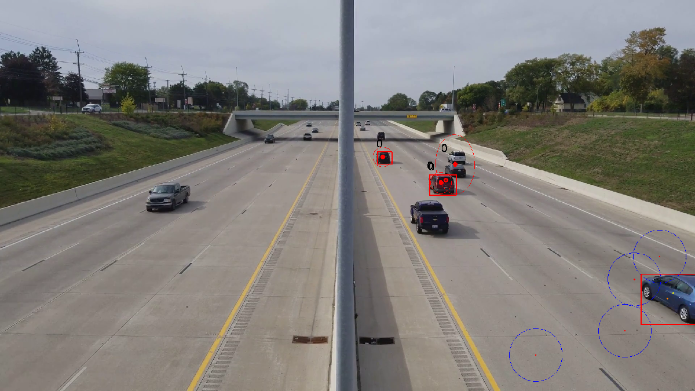
\includegraphics[width=\linewidth]{../../../experiments/E1/V1/SAM/69}
        \caption{Frame number: 69.}
        \label{fig:E1-V1-S2:06}
    \end{subfigure}
    \\
    \begin{subfigure}{0.48\textwidth}
        \centering
        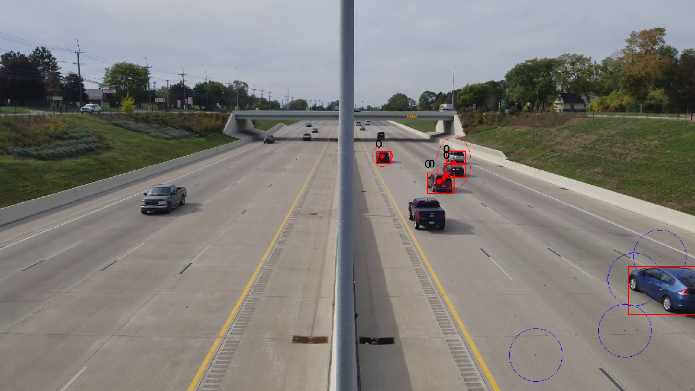
\includegraphics[width=\linewidth]{../../../experiments/E1/V1/SAM/70}
        \caption{Frame number: 70.}
        \label{fig:E1-V1-S2:07}
    \end{subfigure}
    \begin{subfigure}{0.48\textwidth}
        \centering
        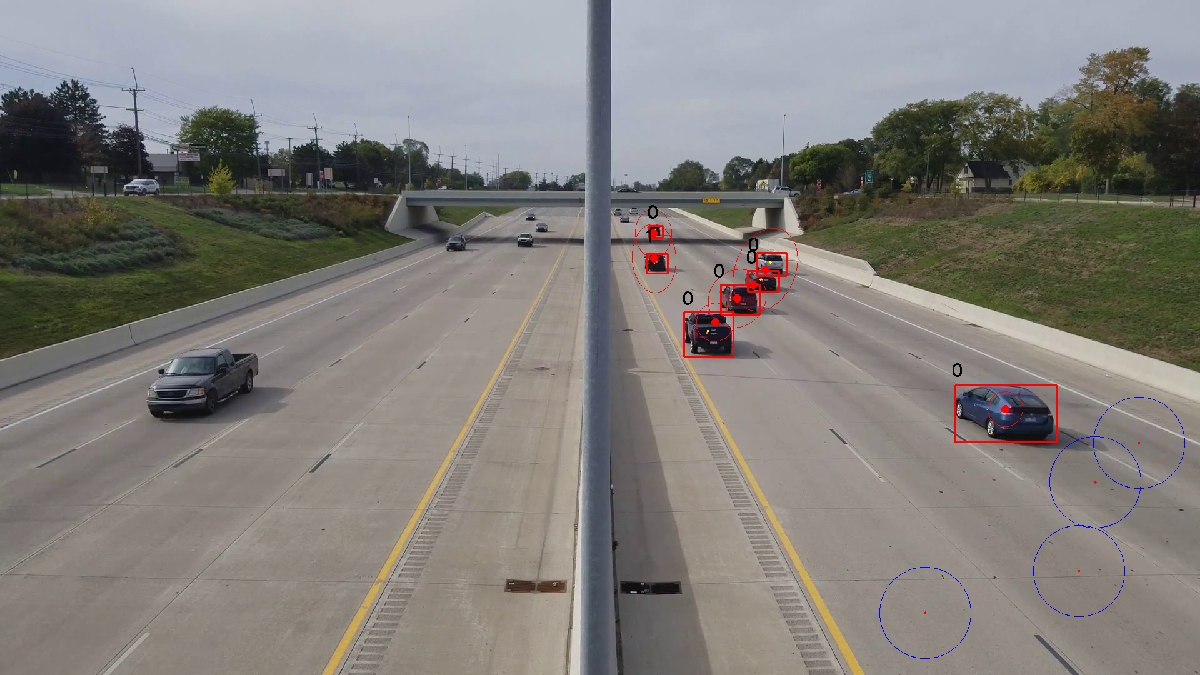
\includegraphics[width=\linewidth]{../../../experiments/E1/V1/SAM/78}
        \caption{Frame number: 78.}
        \label{fig:E1-V1-S2:08}
    \end{subfigure}
    \caption{Image sequence of tracked objects using GM-PHD filter with dynamic detection probability, the YOLO object detector and the SAM image segmentation model.}
    \label{fig:E1-V1-S2}
\end{figure}


\subsubsection{S3 -- Grounded SAM}
The experiment with settings \textit{S3} uses Grounding DINO object detector and the SAM image segmentation model.
All used parameters are included in Table \ref{tab:E1-V1-S3}.
\begin{table}[H]
    \centering
    \begin{tabular}{|c|c|c|c|c|c|c|c|c|c|}
        \hline
        $P_{D,k}(x)$ & $P$ & $\sigma_{\upsilon}$ & $\sigma_{\epsilon}$ & $T_H$ & $T_d$ & $T_p$ & $T_l$ & $T_{text}$ & $T_{bbox}$\\ \noalign{\hrule
        height 1.5pt}
        0.3 & $diag(600,600,600,600)$ & 0.1 & 150 & 1 & 3 & 0.1 & 0.01 & 0.3 & 0.3\\
        \hline
    \end{tabular}
    \caption{The parameter settings for experiment E1-V1-S3 with dynamic detection probability.}
    \label{tab:E1-V1-S3}
\end{table}

Figure \ref{fig:E1-V1-S3} shows the performance of the GM-PHD filter with the dynamic detection probability with settings \textit{S3}.
\begin{itemize}
    \item \textbf{\ref{fig:E1-V1-S3:01}:} Due to the different object detection model, there are more cars detected in the scene. Only four cars drove through the spawn points till this moment, so only there objects are counted to the true count.
    \item \textbf{\ref{fig:E1-V1-S3:02}:} All targets are tracked successfully.
    \item \textbf{\ref{fig:E1-V1-S3:03}:} Unlike YOLO, Grounding DINO is able to detect the arriving car.
    \item \textbf{\ref{fig:E1-V1-S3:07}:} The next arriving car is detected and initialized as well.
    \item \textbf{\ref{fig:E1-V1-S3:08}:} In this frame new problems arises. As cars are far away, closer to each other and the model is still able to detect all cars, we gain too many new targets. For this model, different observation noise is neccessary. Moreover, for these kind of situations, dynamic model and observation noise would be appropriate ssolution.
\end{itemize}

In graph \ref{gr:E1-V1-S3} we see, that the number of detected objects is far beyond the true count. But the number of displayed targets is almost perfect till frame number 66. After that as targets are closer to each other, the number of targets grows rapidly, causing errors to the number of tracked objects.

This settings outperforms the other settings by far. The great performance of Grounding DINO causes another problems arising from characteristics of the video. The video is taken from an angle, which makes cars smaller as they go. This dynamics do go together well with static measurement and observation noise.

\begin{figure}[H]
    \centering
    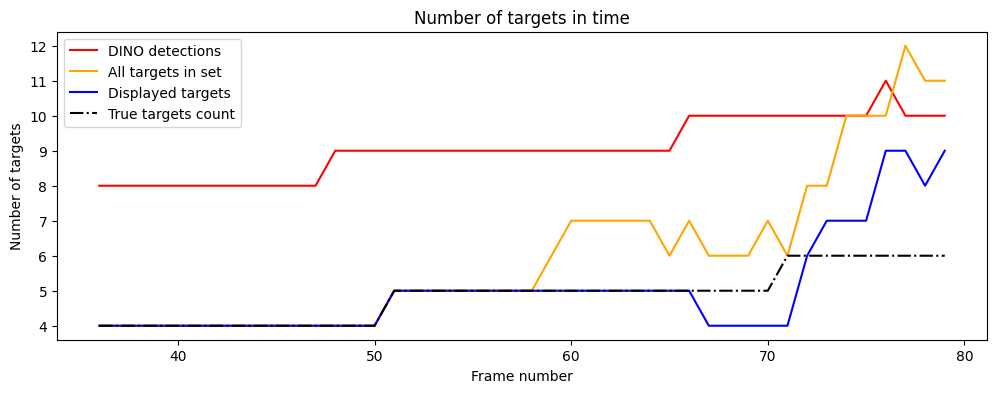
\includegraphics[width=\linewidth]{../../../experiments/E1/V1/DINO/dino_det}
    \caption{Development chart of number of detected targets, targets in filter's queue, displayed targets and true targets' count.}
    \label{gr:E1-V1-S3}
\end{figure}

\begin{figure}[H]
    \centering
    \begin{subfigure}{0.48\textwidth}
        \centering
        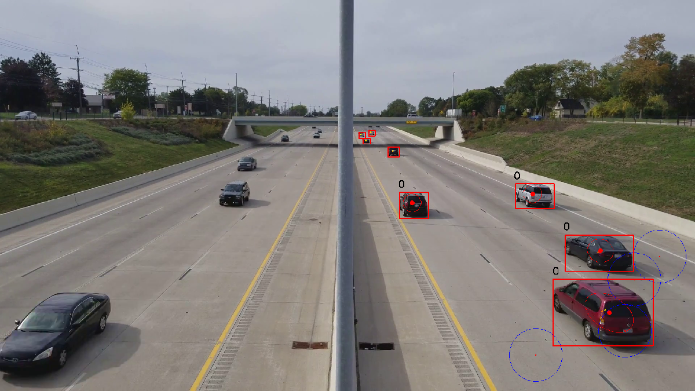
\includegraphics[width=\linewidth]{../../../experiments/E1/V1/DINO/36}
        \caption{Frame number: 36.}
        \label{fig:E1-V1-S3:01}
    \end{subfigure}
    \begin{subfigure}{0.48\textwidth}
        \centering
        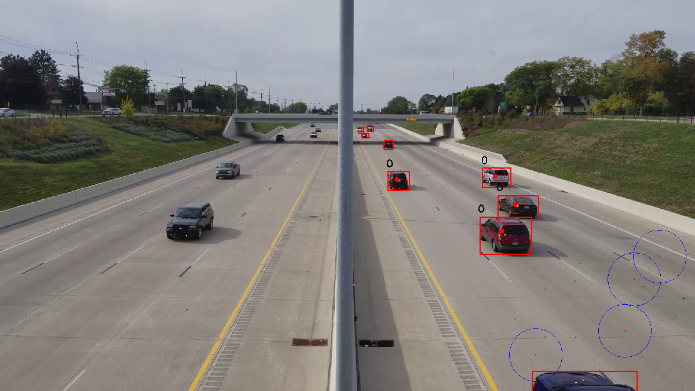
\includegraphics[width=\linewidth]{../../../experiments/E1/V1/DINO/48}
        \caption{Frame number: 48.}
        \label{fig:E1-V1-S3:02}
    \end{subfigure}
    \\
    \begin{subfigure}{0.48\textwidth}
        \centering
        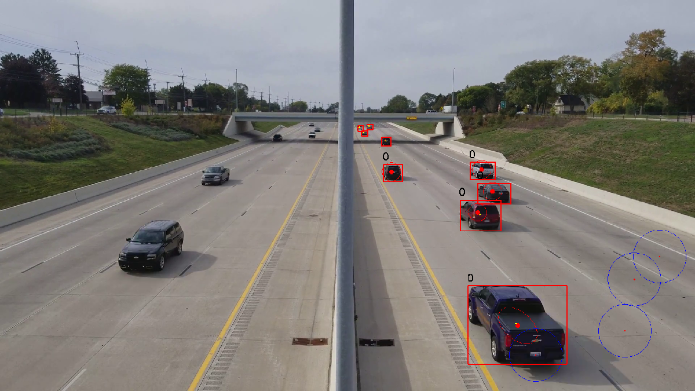
\includegraphics[width=\linewidth]{../../../experiments/E1/V1/DINO/54}
        \caption{Frame number: 54.}
        \label{fig:E1-V1-S3:03}
    \end{subfigure}
    \begin{subfigure}{0.48\textwidth}
        \centering
        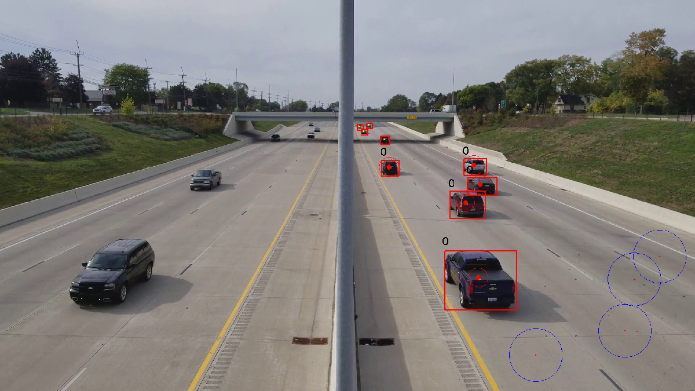
\includegraphics[width=\linewidth]{../../../experiments/E1/V1/DINO/58}
        \caption{Frame number: 58.}
        \label{fig:E1-V1-S3:04}
    \end{subfigure}
    \\
    \begin{subfigure}{0.48\textwidth}
        \centering
        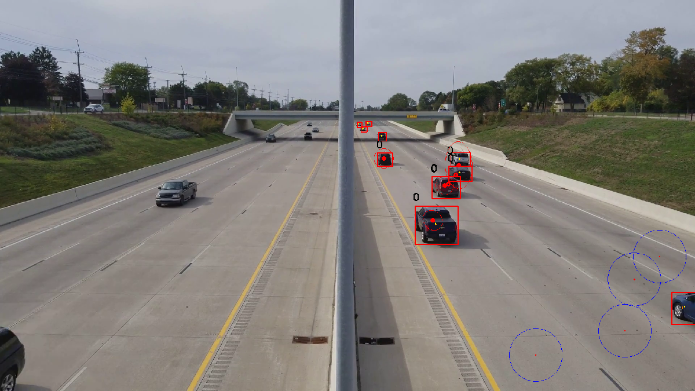
\includegraphics[width=\linewidth]{../../../experiments/E1/V1/DINO/67}
        \caption{Frame number: 67.}
        \label{fig:E1-V1-S3:05}
    \end{subfigure}
    \begin{subfigure}{0.48\textwidth}
        \centering
        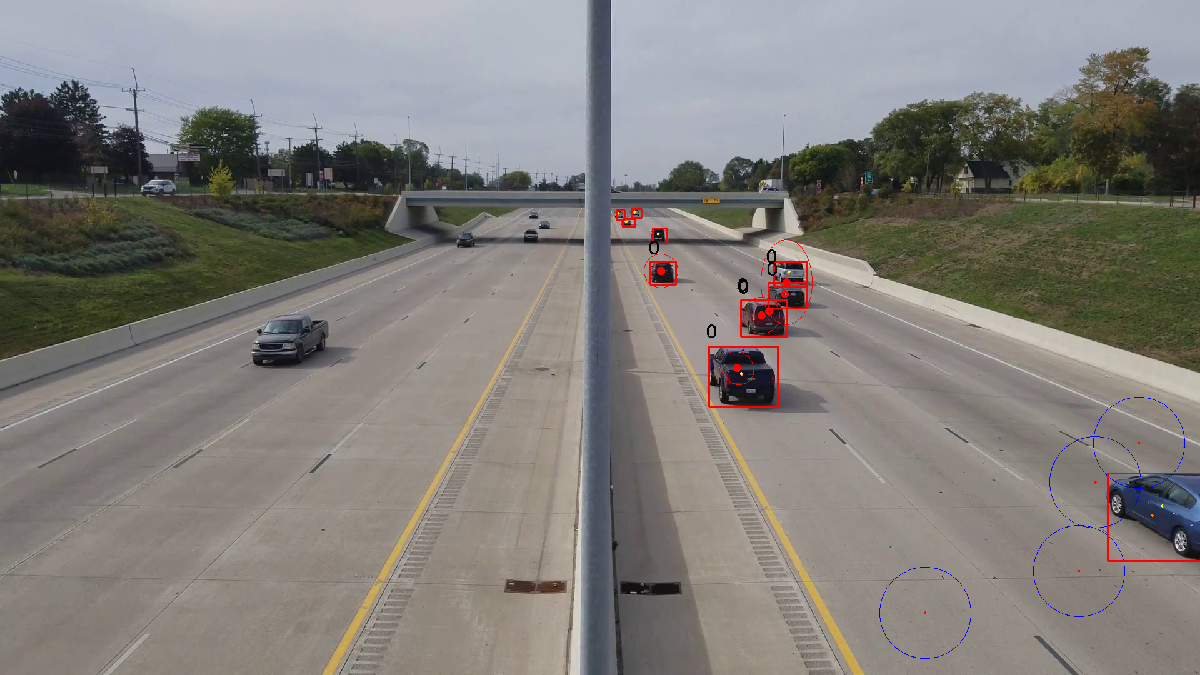
\includegraphics[width=\linewidth]{../../../experiments/E1/V1/DINO/69}
        \caption{Frame number: 69.}
        \label{fig:E1-V1-S3:06}
    \end{subfigure}
    \\
    \begin{subfigure}{0.48\textwidth}
        \centering
        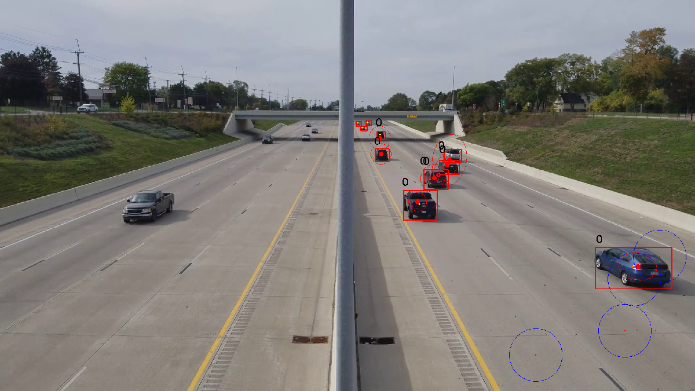
\includegraphics[width=\linewidth]{../../../experiments/E1/V1/DINO/73}
        \caption{Frame number: 73.}
        \label{fig:E1-V1-S3:07}
    \end{subfigure}
    \begin{subfigure}{0.48\textwidth}
        \centering
        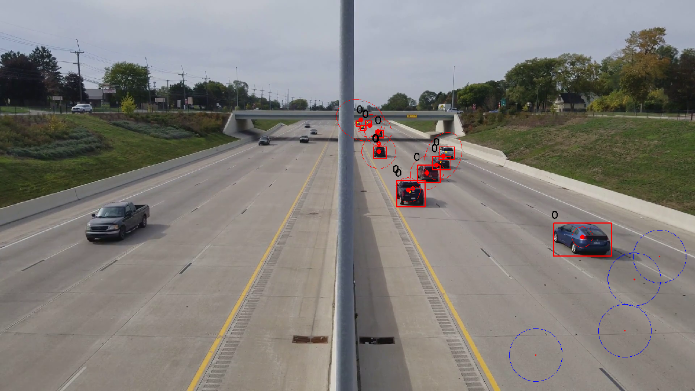
\includegraphics[width=\linewidth]{../../../experiments/E1/V1/DINO/78}
        \caption{Frame number: 79.}
        \label{fig:E1-V1-S3:08}
    \end{subfigure}
    \caption{Image sequence of tracked objects using the GM-PHD filter with the dynamic detection probability and the Grounded DINO model.}
    \label{fig:E1-V1-S3}
\end{figure}
